\documentclass{article}
\usepackage{tikz}
\usetikzlibrary{automata, positioning}

\begin{document}

\begin{center}
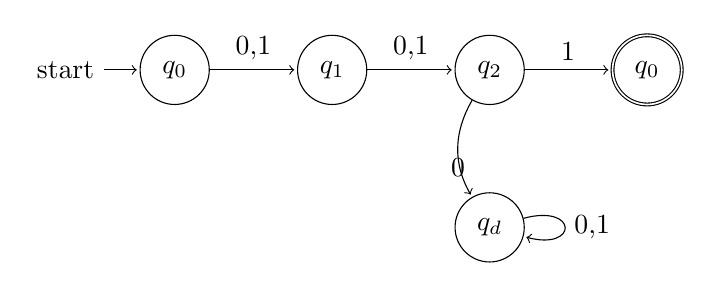
\begin{tikzpicture}[shorten >=1pt, node distance=2cm, on grid, auto] 

   \node[state, initial] (q0)   {$q_0$}; 
   \node[state] (q1) [right=of q0] {$q_1$}; 
   \node[state] (q2) [right=of q1] {$q_2$}; 
   \node[state, accepting] (q3) [right=of q2] {$q_0$}; 
   \node[state] (qd) [below=of q2] {$q_d$}; 

   \path[->] 
    (q0) edge node {0,1} (q1)
    (q1) edge node {0,1} (q2)
    (q2) edge node {1} (q3)
         edge [bend right] node[below] {0} (qd)
    (qd) edge[loop right] node {0,1} (qd);

\end{tikzpicture}
\end{center}

\end{document}
